% !TEX root = hazel-LIVE2018.tex

\section{Live Palettes}
\label{sec:palettes}


\begin{figure}[t]
\vspace{-4px}
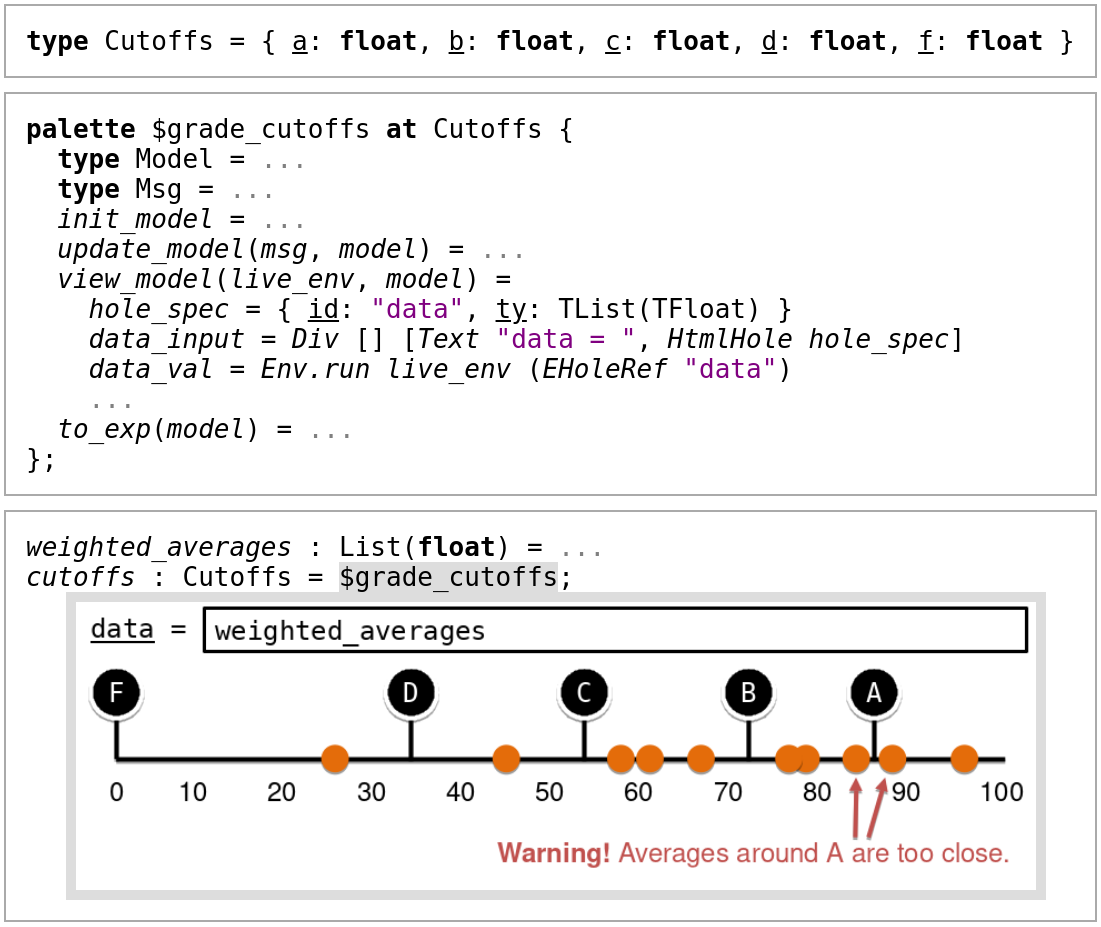
\includegraphics[width=0.7\textwidth]{images/cutoffs-new.png}
\caption{An example where the teacher assigns cutoffs 
for letter grades using a domain-specific live palette.}
\label{fig:cutoffs-example}
\vspace{-4px}
\end{figure}

Another editor service that we are designing for integration into \Hazel 
is the \emph{live palette} service.
Palettes, which were introduced in work on
\emph{active code completion} by \citet{ActiveCodeCompletion},  allow programmers to fill typed 
holes by directly manipulating specialized graphical user interfaces rather than by exclusively entering symbolic
code. For example, a palette might allow the programmer to 
fill in a hole of type \li{Color} using a color selection  
user interface, rather than by construcing a \li{Color} value  
using the constructors of that type. \citet{ActiveCodeCompletion} elicited a large number of other
examples of data types where an alternative, graphical 
method of constructing a value of a particular type might be
useful. Due to the large number of examples, the system in that paper, called {Graphite}, is designed to be extensible by library providers. 

Palettes in {Graphite} 
are ephemeral, operating as a form of code completion, but projectional editors, e.g. Barista \cite{ko_barista:_2006} and \li{mbeddr} \cite{voelter_mbeddr:_2012}, often support a small fixed number of  
palettes (there called \emph{projections}) that persist, i.e. that appear within the code itself. 
Projectional palettes also improve upon Graphite's palettes in that they are compositional, i.e. they allow code to appear within holes that appear inside the palette (e.g. the entries in a matrix palette). 

Like Graphite, \Hazel's palette system is extensible. 
Like projectional palettes, \Hazel's palettes are also persistent and compositional. 
Holes that appear inside palettes
are governed by a hygiene discipline based on recent work on splicing in user-defined literal macros
\cite{tlms-icfp18}. 
Uniqely, \Hazel's palette system is live: the program 
can be executed before the palette has generated code
and the hole closures associated with the hole that the 
palette is tasked with filling can be used by the palette
to provide concrete feedback to the programmer.

Let us consider an illustrative example that demonstrates
all of these qualities. 

Fig.~\ref{fig:cutoffs-example} shows a palette that allows the teacher to determine grade cutoffs by dragging markers visually along a number line, with the student's grades superimposed.

%
Each palette is required to implement a
Model-Update-View interface, following roughly the Elm architecture \cite{ElmArchitecture}. 
In the function \li{view} that generates the user
interface, the palette may request that a nested hole be
rendered using the \li{HtmlHole} constructor, choosing a
name for it (\li{id}) and specifying its type (\li{ty}). When the cursor is in this hole, the editor (Hazel) provides all of the usual editor services based on the specified type. Here, the \li{data} hole 
is filled by an expression \li{weighted_averages} of type \li{list(float)} (from the example in \autoref{fig:intro-example}, extended with some additional student data). This would have been suggested by Track 3.
%% for it (\li{hole\_spec.id}) and specifying its type
%% (\li{hole\_spec.type}).
%

At any point, the editor may invoke the palette's
\li{to_exp} function to produce the expansion, \ie{}~an expression
represented as a value of type \li{expr_ast}. The palette can refer to
the nested hole abstractly (via \li{id}) 
%% the nested hole abstractly (via its \li{hole\_spec.id})
with the \li{EHoleRef} constructor, allowing its filled
expression to be used abstractly (at type \li{ty}). The \li{to_exp} function generates a value of type \li{grade_cutoffs},
shown in \autoref{fig:intro-example-part-2}, based on the positions of the grade markers,
which can be dragged by the user. The position of these markers is tracked in the model. The palette is implemented such that manipulating any one of the cutoffs also causes the others to change if the sorting invariant would have been violated.

The palette can ask the environment to evaluate the expression
 inside a hole by referring to it abstractly and calling \li{Env.run} as shown in the body 
 of the \li{view} function. Here, the palette uses this to show orange dots for all of 
 the computed weighted averages. The palette also runs a bucketing calculation (not shown)
based on the data and the current cutoffs, and then checks
the data-driven ``fairness'' criterion that no two students
whose grades are within some small factor get assigned
different letter grades. This allows the teacher to easily choose appropriate points, and demonstrates the utility of a palette over a plain expression. 
% cutoffs and is usable for different data sets in different
% courses and in different years.
 If the hole was not filled or filled by an indeterminate value, then 
 the dots and warning would not be displayed.
